\chapter{Implementation}
\label{chapter:implementation}

This chapter describes the theoretical aspects of six-axial optical force sensor development, the data filtration, communication protocols and the calibration process?

% ~\nameref{capter:literature_review}


% \chaptermark{capter:literature_review}
% This chapter covers theoretical aspects related to the translation of Java to EO, developed projections, and a description of the software project developed alongside this thesis.


% \section{Conceptual comparison of Java and EO}
% \label{section:conceptual_comparison}

% To start translating of one language into another, it is important to understand their differences. Even the same term may be interpreted differently by developers of several languages.

% \subsection{Paradigm}

% It is important to remember that in the past various languages, including Java, spoiled the original notion of the object-oriented paradigm. Thus, the object-oriented paradigm is interpreted differently by developers of different languages. Original implementation of object-oriented paradigm is present in Smalltalk \cite{smalltalk} and is focused on objects, not classes.

% Java implements a nowadays traditional OOP paradigm. The correct name of the paradigm would be \emph{class-oriented}, since developer has no access to objects, only to classes. This approach also strictly forces developers to put everything in classes or interfaces, which are the only available top-level constructs.

% EO is closer to the functional paradigm, with a focus on objects, as in the original object-oriented paradigm.

% \subsection{Visibility}
% % TODO: wrap this into some section/subsection.
% % TODO: maybe move part of this stuff to the EO overview chapter?
% Java has a strict visibility system that includes four levels described in
% subsection \ref{subsection:java_visibility}. EO, on the other hand, has no
% visibility system at all. Such a visibility system is hardly possible in EO given its dynamic nature, including dynamic typing, lack of object structure specification and unlimited access to the creation and modification of objects.
% These features are required to keep the language structure flexible enough to translate various languages into it.


% \subsection{Mutability}
% In Java, all variables are mutable by default (though it may be limited using final). EO has no built-in mutability, but it has workarounds for that in the standard library: \ff{memory} and \ff{cage}.


% \subsection{Programming style}
% Java has an imperative style --- developer writes a code that describes \emph{how} to do the task. Declarative style may be achieved using custom-implemented pair of executor and data structure, but it will not work soundly with libraries (both standard library and external libraries). Custom wrappers are needed to support libraries.

% EO has a declarative style --- developer writes \emph{what they want to achieve}, not how to achieve that. Imperative style may be achieved using a built-in atom named \ff{seq}, but because of the implementation nature, the scope of \ff{seq} is more restrictive than the object scope, e.g., it is not possible to declare variables inside.



% \section{Projections}

% This section will go over theoretical approaches of projecting Java source code into semantically equivalent EO source code.

% \subsection{Naming}
% Java and EO have different conventions for naming language components, and while Java does not enforce naming conventions, EO does. Consequently, name mapping has to be developed and be consistent across the translator to keep the result code working.

% Specifically: object and attribute names in EO can only start with lower-case letters and continue with upper/lower case letters, numbers, dashes or underscores. This differs from Java only in the first symbol, therefore, the solution is to prepend names with fixed text sequence.

% Also, EO has problems with attribute shadowing. Attribute shadowing is a feature of a language that allows redefining variables (attributes in EO terms) in nested scopes. This feature works in an unpredictable manner, especially considering the unstable nature of EO (it is still in the early stage of development and behavior changes frequently as of the time of writing this). Because of that, the translator avoids name duplication as much as possible. The first step to minimize such duplications is to prepend different types of source code tokens with different prefixes.

% As a solution to the attribute shadowing problem, the following mappings were developed:
% \begin{itemize}
%     \item class names are prepended with \texttt{class\_\_}
%     \item variables are prepended with \texttt{var\_\_}
%     \item arguments are prepended with \texttt{arg\_\_}
%     \item methods are prepended with \texttt{method\_\_}
% \end{itemize}


% \subsection{Constructors}
% Java, like many modern OOP languages, has class constructors. EO does not have classes, and thus the implementation of constructors is under full control of the translator. In the current form, Java constructors are mapped into function attributes with an extra \texttt{cons} name.


% \subsection{Overloading}
% Also, EO does not support method/constructor overloading and even does not have functions directly. They are simple objects, like everything in the language. Therefore, the name of methods/constructors are appended with type names, separated with \texttt{\_\_}. Generics information is omitted, as JVM does not have it as well.

% Example of resulting mapping considering everything above:
% \begin{ffcode}
% class A {
%   A(int member) {...}
%   void functionName(int arg1, Option<Value> arg2) {...}
% }
% \end{ffcode}

% \begin{ffcode}
% [] > class__A
%   [] > new
%     [] > this
%       [var__member] > cons__int
%         ...

%       [] > method__functionName__int__Option
%         ...
% \end{ffcode}


% \subsection{Expressions}
% Java provides a way to create complex nested and chained (separated with dot) expressions. These expressions can cause various side-effects in various order. 


% \subsubsection{Chained expressions}

% The tricky case is chained expressions. Due to EO's specific function calling approach, calling a method of a class instance requires passing that instance as the first argument, i.e. \texttt{obj.function(obj)}. This is effortless when single-expression statements are used, but chaining with a dot requires storing the intermediate object somewhere to be able to proceed in the chain.

% Consider the following Java example:

% \begin{ffcode}
%   var result = obj.setValue(value).computeResult();
% \end{ffcode}

% Here, \texttt{obj} should be passed between chained calls. To resolve this collision, it was decided to split each chain operation into a separate binding, and use them inside other bindings. This allows to abstract out the double use of the same value from higher-level abstraction. 

% Since internal operations do not act as dependencies to the outside of expression, their names are generated randomly and have a UUID format.

% The order goes from inside to outside, so dependencies of outer expression parts are already defined above, although it does not matter to EO, as an evaluation only starts in the \texttt{seq} block at the end of the function object.


% The example of EO code that corresponds to the above Java snippet:

% \begin{ffcode}
% ... > obj
% ... > value
% ...
% [obj] > <uuid_1>
%   seq > @
%     obj.setValue obj value
% [obj] > <uuid_2>
%   seq > @
%     obj.computeResult obj
% ...
% seq > @
%   ...
%   <uuid_2>
%     <uuid_1>
%       obj
% \end{ffcode}

% Although the EO variant takes considerably more code to do the same operation, the language was never meant for hand-writing code, only for translation from other languages.


% \subsubsection{Side-effects in expressions}

% Consider the following Java snippet:

% \begin{ffcode}
% var out = obj.setValue(obj2.setValue(obj2.getCount()).i++);
% \end{ffcode}

% It is different from the previous snippet by one feature --- post-increment operation, which is an in-place mutating side-effect.

% In this code, in given order, the following operations occur:
% \begin{itemize}
%     \item Function \texttt{getCount} of \texttt{obj2} is invoked and result is obtained 
%     \item Function \texttt{setValue} of \texttt{obj2} is invoked with the obtained value
%     \item \texttt{obj2} returns itself for further chained call
%     \item Property \texttt{i} of \texttt{obj2} is obtained
%     \item Property \texttt{i} of \texttt{obj2} is incremented by 1
%     \item Function \texttt{setValue} of \texttt{obj} is invoked with value obtained before increment, as this is value type, not reference type
%     \item The result of \texttt{setValue} is assigned to \texttt{out}
% \end{itemize}

% As it is seen from the list above, the order of execution does not correspond to the AST, in particular --- post-increment operation. This operation should have been placed before obtaining the result, as in pre-increment, to match the AST structure. This fact of altered order makes Java code hard to translate to EO, which does not have corresponding syntactic sugar, as well as value-typed variables.

% The general problem is causing side-effects from the expression: EO discourages any side-effect operations and only provides "gray" workaround atoms to mimic side-effects, to create a compatibility layer with side-effect-based programs. But since there are still no value types, we have to work around operations that rely on them with custom logic (i.e., creating a new variable).

% Considering methods described above, we can obtain the following EO mapping:

% \begin{ffcode}
% ... > obj
% ... > obj2
% ...
% [obj] > <uuid_1>
%   memory > result
%   seq > @
%     result.write
%       obj.getCount obj
%     result
% [obj arg] > <uuid_2>
%   seq > @
%     obj.setValue obj arg
% [obj] > <uuid_3>
%   memory > result
%   seq > @
%     result.write
%       obj.i
%     obj.i.write
%       add
%         obj.i
%         1
%     result
% [obj arg] > <uuid_4>
%   seq > @
%     obj.setValue
%       obj
%       arg
% ...
% seq > @
%   ...
%   <uuid_4>
%     obj
%     <uuid_3>
%       <uuid_2>
%         obj2
%         <uuid_1>
%           obj2
%   ...
% \end{ffcode}


% Notice how post-increment was implemented in \texttt{<uuid\_3>}: new \texttt{memory} object (think of it as of cell that can store some value) is created, the current value is copied there, and then the original object's value is updated.

% The same approach is used everywhere where value types are used (for Java, the list includes \texttt{int}, \texttt{long}, \texttt{short}, \texttt{char}, \texttt{float}, \texttt{double}). In this case, it is used in \texttt{<uuid\_1>}. This provides a reliable way to ensure that the original value will not be changed by subsequent function calls, as it is not changed in Java.


% \subsection{Resolving Java compound names}
% Java has a very unfortunate feature of referencing nested classes/members: every token is separated with a dot in any case. Therefore, it is impossible to tell which exact operation is represented by a particular dot: is it a part of a package name, referencing a class from a package or referencing a member of a class.

% To determine the operation of the compound name, the import block is analyzed:
% if the line from the Java import block (excluding the last part, either \texttt{*} or class name) is a start of the compound name, parts of the package are not altered in the EO compound name; the file referenced by the package name is loaded, parsed and analyzed. parts that correspond to class names are prepended with \texttt{class\_\_}, parts that correspond to variable names are prepended with \texttt{var\_\_}.


% \subsection{Mapping classes}
% % <insert reference to conference paper>
% % <copy from J2EO paper>

% Class bodies are fairly straightforward to translate.
% \begin{itemize}
%     \item class is an object with all static members and static methods, plus \texttt{new} object factory and \texttt{cons<n>} constructors. It also decorates the superclass, inheriting its static members and methods.
%     \item \texttt{new} method decorates superclass'es \texttt{new} object and defines class members with their default values over that.
%     \item \texttt{cons<n>} method that contains corresponding Java constructor code.
% \end{itemize}

% What poses a challenge is an inheritance, especially multiple inheritance (implemented via interfaces in Java). There are still no observed approaches to map interfaces in the project, so they will be skipped for the time being. The focus will be on mapping classes.

% Superclass is written to \texttt{super} attribute of an instance during its creation.


% Below is an example of class mapping:

% Original Java code snippet:
% \begin{ffcode}
% class A {
%   int i = 42;
%   int getI() { return i; }
% }
% class B extends A {
%   int i = 1;
%   B() { super(); i = 2; }
%   int getI() { return i; }
%   int getSuperI() { return super.i; }
%   int setSuperI(int i) { super.i = i; }
% }
% \end{ffcode}

% Produced semantically-equivalent EO code:
% \begin{ffcode}
% [] > class__A
% [] > new
%   [] > this
%     memory > i
%     [this] > getI
%       this.i > @
%   seq > @
%     this.i.write 42
%     this
% [this] > cons1
%   this > @

% [] > class__B
% [] > new
%   [] > this
%     class__A.new > super
%     super > @
%     memory > i
%     [this] > getI
%       this.i > @
%     [this] > getSuperI
%       this.super.i > @
%     [this i] > setSuperI
%       seq > @
%         this.super.i.write i
%         this
%   seq > @
%     this.i.write 1
%     this
% [this] > cons1
%   class__A.cons1 this > this2
%   seq > @
%     this2.i.write 2
%     this2
% \end{ffcode}


% \subsection{Mapping interfaces}

% EO's feature that allows the extension of other objects is decoration. Decoration only allows simulation of singular inheritance, though. Java 8 brought default methods to interfaces --- which essentially facilitated multiple inheritance. This does not fit into $\varphi$-calculus, so can only be worked around, not natively implemented.

% The current solution simply ignores interfaces, since mostly they only facilitate static checking when data hiding is needed. This approach behaves incorrectly with default methods, though.


% \section{J2EO implementation overview}

% In addition to theoretical mappings, the result of work on the thesis is a software project named J2EO. The project is written in Java/Kotlin with parser implemented in ANTLR \cite{antlr_website}. 

% The flow of a single Java file through different modules is shown below.

% \begin{figure}[H]
%   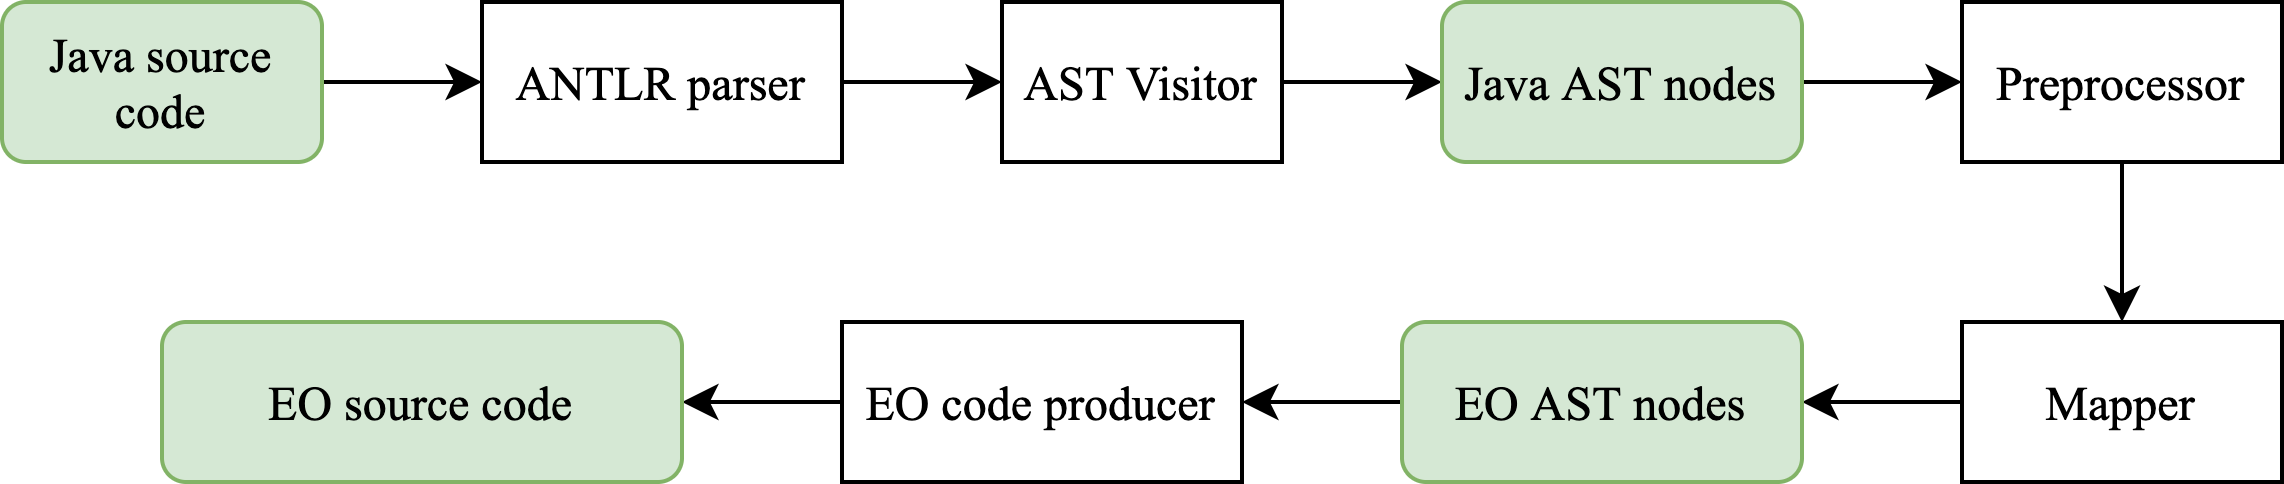
\includegraphics[width=1\textwidth]{j2eo_structure.png}
%   \centering
%   \caption{Processing of a single Java file through the J2EO pipeline}
%   \label{fig:j2eo_flow}
% \end{figure}

% The wrapper that handles I/O, execution of pipeline and other routine tasks is not covered by this text.

% The following part of the section describes each of the steps in more detail.

% \subsection{ANTLR parser}
% Java parsers for modern versions of the language are hardly available on the Internet. The only parser that fully covers Java 17 is implemented in ANTLR and is available on GitHub \cite{antlr_java_parser}. Slight modifications are required to make it work for J2EO's use case.

% \subsection{AST Visitor}
% This pipeline step executes ANTLR parser and visits each node to generate an internal Java AST node. This step is required because ANTLR itself does not generate AST nodes, it only provides context which can be used to obtain parts of the tree.

% \subsection{Preprocessor}

% The preprocessor applies naming convention patches to the code. This step includes prefixing of identifiers, renaming imports to suit EO conventions and other semantically-neutral changes.

% \subsection{Mapper}

% This is the core pipeline step, which produces EO AST nodes from preprocessed Java AST nodes. The methodology of projection of AST nodes is provided in the above section.

% \subsection{EO code producer}

% The final step of the pipeline is to produce source code from the EO AST. This part is implemented as Kotlin extension functions which add methods to EO AST nodes in a non-invasive manner.

% \subsection{Summary}

% All pipeline steps above are implemented in a functional style. Thus, none of the functions utilize the shared mutable state, which makes it possible to parallelize the translation of files. The parallel version of J2EO was successfully tested.

% J2EO project is open-source and is available on GitHub \cite{j2eo_repo}. Anybody can use it and contribute to it.




